\documentclass[ignorenonframetext,a4paper]{beamer}
\setbeamertemplate{caption}[numbered]
\setbeamertemplate{caption label separator}{: }
\setbeamercolor{caption name}{fg=normal text.fg}
\beamertemplatenavigationsymbolsempty
\usepackage{lmodern}
\usepackage{amssymb,amsmath}
\usepackage{ifxetex,ifluatex}
\usepackage{fixltx2e} % provides \textsubscript
\ifnum 0\ifxetex 1\fi\ifluatex 1\fi=0 % if pdftex
  \usepackage[T1]{fontenc}
  \usepackage[utf8]{inputenc}
\else % if luatex or xelatex
  \ifxetex
    \usepackage{mathspec}
  \else
    \usepackage{fontspec}
  \fi
  \defaultfontfeatures{Ligatures=TeX,Scale=MatchLowercase}
\fi
\usetheme[]{Padova}
% use upquote if available, for straight quotes in verbatim environments
\IfFileExists{upquote.sty}{\usepackage{upquote}}{}
% use microtype if available
\IfFileExists{microtype.sty}{%
\usepackage{microtype}
\UseMicrotypeSet[protrusion]{basicmath} % disable protrusion for tt fonts
}{}
\newif\ifbibliography
\hypersetup{
            pdfborder={0 0 0},
            breaklinks=true}
\urlstyle{same}  % don't use monospace font for urls
\usepackage{longtable,booktabs}
\usepackage{caption}
% These lines are needed to make table captions work with longtable:
\makeatletter
\def\fnum@table{\tablename~\thetable}
\makeatother
\usepackage{graphicx,grffile}
\makeatletter
\def\maxwidth{\ifdim\Gin@nat@width>\linewidth\linewidth\else\Gin@nat@width\fi}
\def\maxheight{\ifdim\Gin@nat@height>\textheight0.8\textheight\else\Gin@nat@height\fi}
\makeatother
% Scale images if necessary, so that they will not overflow the page
% margins by default, and it is still possible to overwrite the defaults
% using explicit options in \includegraphics[width, height, ...]{}
\setkeys{Gin}{width=\maxwidth,height=\maxheight,keepaspectratio}

% Prevent slide breaks in the middle of a paragraph:
\widowpenalties 1 10000
\raggedbottom

\AtBeginPart{
  \let\insertpartnumber\relax
  \let\partname\relax
  \frame{\partpage}
}
\AtBeginSection{
  \ifbibliography
  \else
    \let\insertsectionnumber\relax
    \let\sectionname\relax
    \frame{\sectionpage}
  \fi
}
\AtBeginSubsection{
  \let\insertsubsectionnumber\relax
  \let\subsectionname\relax
  \frame{\subsectionpage}
}

\setlength{\parindent}{0pt}
\setlength{\parskip}{6pt plus 2pt minus 1pt}
\setlength{\emergencystretch}{3em}  % prevent overfull lines
\providecommand{\tightlist}{%
  \setlength{\itemsep}{0pt}\setlength{\parskip}{0pt}}
\setcounter{secnumdepth}{0}
\usepackage{booktabs}
\usepackage{subfig}
\usepackage{multicol}
\usepackage{rotating}
\usepackage{mathtools}
\usepackage{pgfplots}
\usepackage{listings}
\usepackage{multirow}
\usepackage{amssymb}
\usepackage{pifont}
\usepackage{tikz}
\usepackage{graphics}
\usepackage{hyperref}
\usepackage{enumerate}
\hypersetup{ colorlinks = true, linkcolor = blue, filecolor = magenta, urlcolor = cyan,}

\title{\Large\textbf{Regression Models and Survival Analysis in the Bayesian context}}
\subtitle{\large\textbf{\textrm{IBIG 2018}}}
\author{\centering\underline{\textbf{Daniele Bottigliengo}}\thanks{\tiny Unit of Biostatistics, Epidemiology and Public Health, Department of \newline Cardiac, Thoracic, Vascular Sciences and Public Health, University of Padua, Italy}}
\date{\centering\emph{Padova, Italy, November 22, 2018}}

\begin{document}
\frame{\titlepage}

\begin{frame}{Build a Bayesian model}

How to build a model in the Bayesian context?

\begin{itemize}
\item
  Statistical modeling can be viewed as the process of setting up a
  model for the data generating process
\item
  The main interest is to draw conclusions on some quantities of
  interest that are unknown (parameters) conditioning on quantities that
  are known and observed (observed data)
\item
  In a Bayesian framework, it means expressing the uncertainty in the
  unknown quantities by using probability distributions, i.e.
  \emph{posterior} distributions
\item
  \emph{Posterior} distributions are derived by combining external
  information on the parameters in the form of \emph{prior}
  distributions and observed information in the form of the
  \emph{likelihood}
\end{itemize}

\end{frame}

\begin{frame}{Two sorts of Bayesian analyses}

Two types of Bayesian data analysis can be identified (Gelman, Simpson,
and Betancourt 2017):

\begin{enumerate}
\setlength\itemsep{1em}
 \item{\textbf{Ideal analysis}}
    \begin{itemize}
    \item{Prior defined before the data are observed}
    \item{Data are analyzed and prior is update}
    \end{itemize}
 \item{\textbf{Analysis with default priors}}
    \begin{itemize}
    \item{Data are retrieved and a model with some or many parameters
          is constructed}
    \item{Priors are then defined to carry on the inference process}
    \end{itemize}
\end{enumerate}

\end{frame}

\begin{frame}{The role of the priors (1)}

\begin{itemize}
\item
  The second type of analysis is concerned with defining priors that are
  somewhat linked with the likelihood (observed data)
\item
  Such priors can be thought as \textbf{regularizing} priors and they
  are designed to make more stable inference
\item
  \emph{Weakly informative} priors are distributions that can accomplish
  regularized inference and may be used as the default starting point
\end{itemize}

\end{frame}

\begin{frame}{The role of the priors (2)}

\begin{itemize}
\item
  The prior can play a very important role during model building,
  especially if the data are complex and noisy
\item
  It is important to calibrate prior distributions to obtain reasonable
  answers given the analyzed situation
\item
  A robust workflow must be implemented to create a solid model:

  \begin{itemize}
  \tightlist
  \item
    potential observed data given particular priors
  \item
    discrepancies between potential and actual observed data
  \end{itemize}
\end{itemize}

\end{frame}

\begin{frame}{Bayesian workflow}

\includegraphics[width = 1.1\linewidth]{figures/bayesian_workflow.png}

\end{frame}

\begin{frame}{1) Exploratory Data Analysis}

It should be the starting point of every statistical analyses (Gelman
2004):

\begin{itemize}
\setlength\itemsep{1em}
  \item{Plot the distribution of observed data}
  \item{Inspect possible relationships between outcome and potential
        predictors}
  \item{Look for patterns beyond what is expected}
  \item{Study missing data}
\end{itemize}

\end{frame}

\begin{frame}{1) Exploratory Data Analysis}

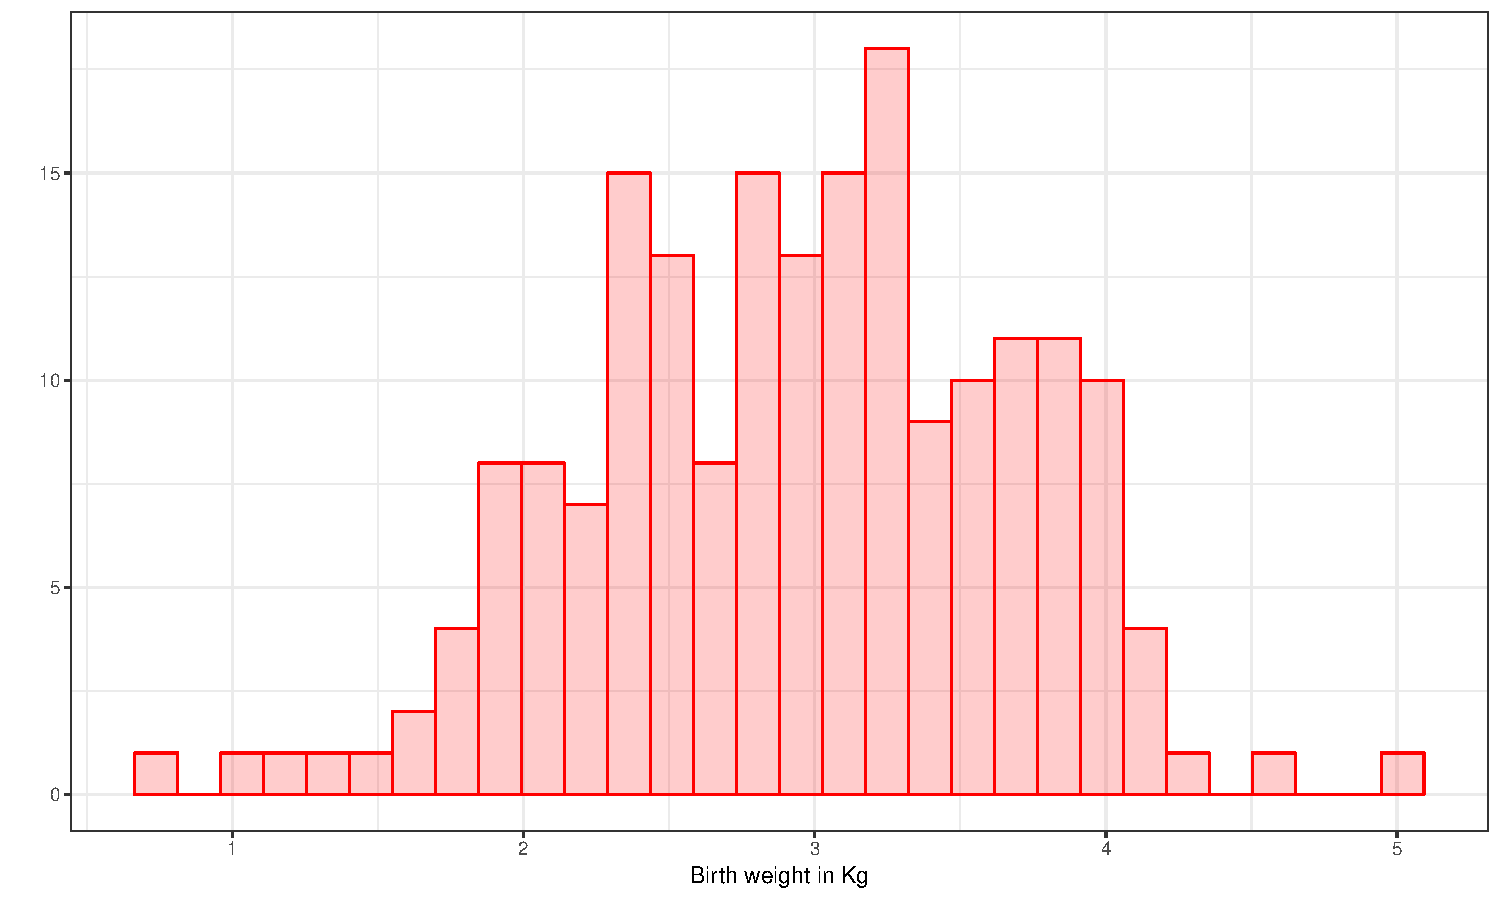
\includegraphics{DB_presentation_slides_files/figure-beamer/unnamed-chunk-2-1.pdf}

\end{frame}

\begin{frame}{1) Exploratory Data Analysis}

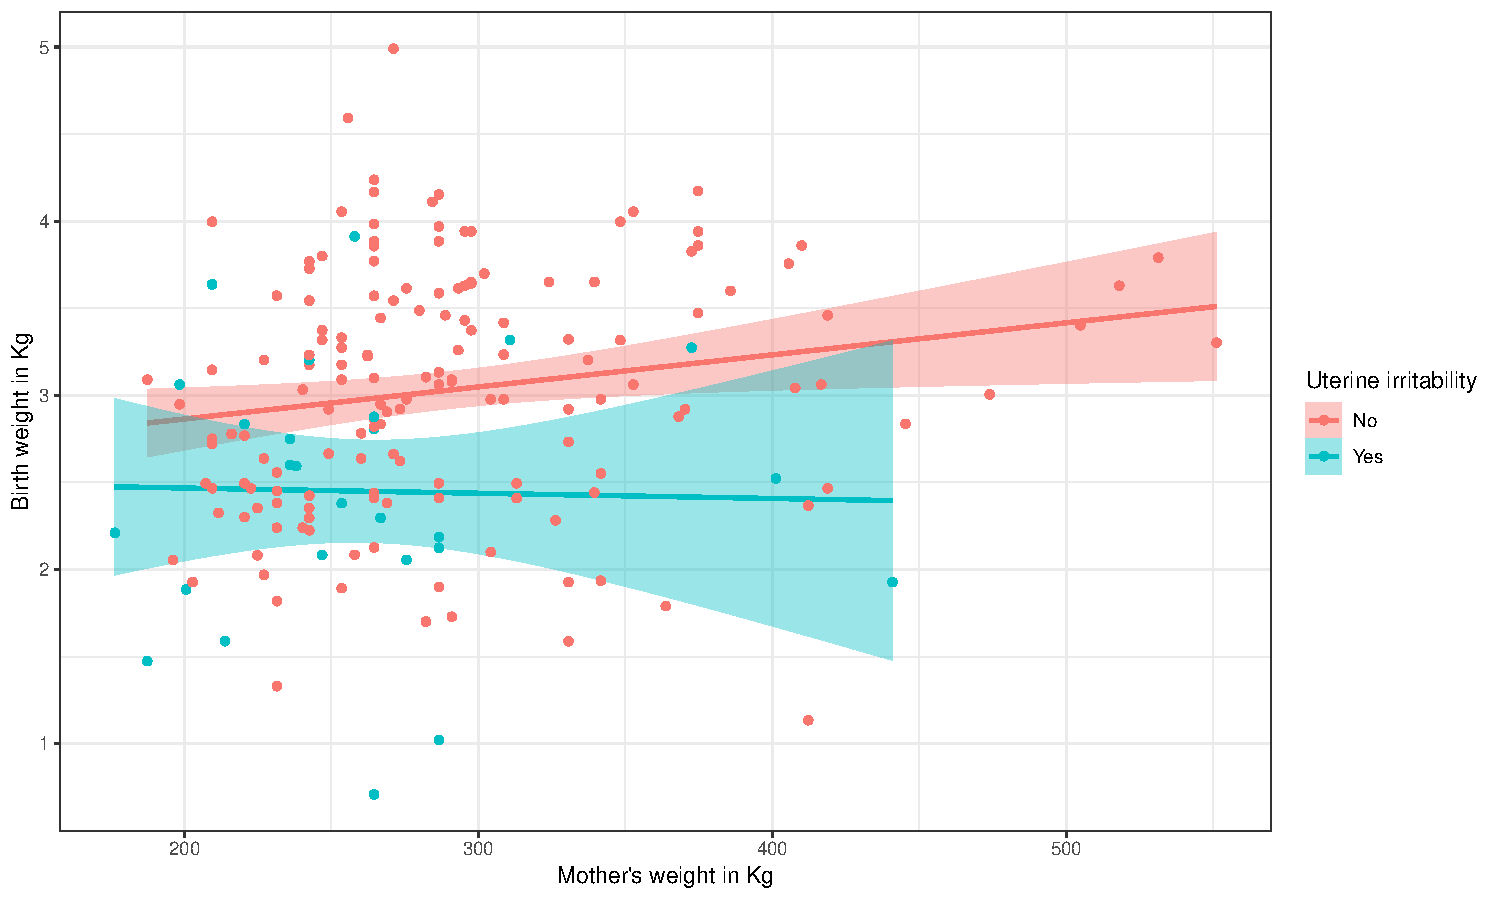
\includegraphics{DB_presentation_slides_files/figure-beamer/unnamed-chunk-3-1.pdf}

\end{frame}

\begin{frame}{1) Exploratory Data Analysis}

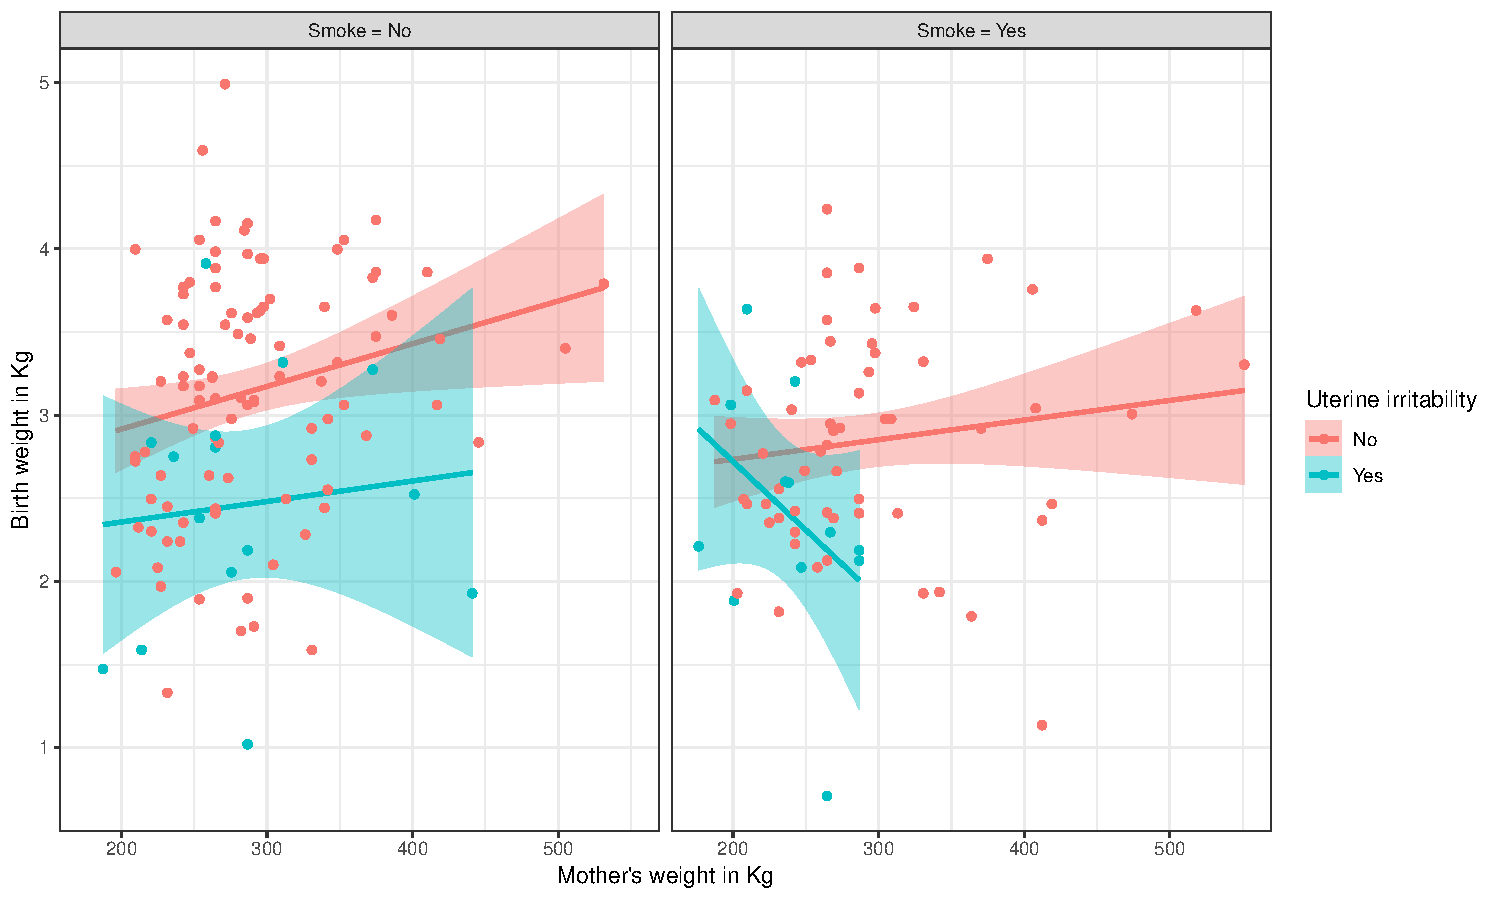
\includegraphics{DB_presentation_slides_files/figure-beamer/unnamed-chunk-4-1.pdf}

\end{frame}

\begin{frame}{2) Data simulation}

\begin{itemize}
\setlength\itemsep{1em}
  \item{The use of simulated data can be very helpful to understand
        the model the analyst is going to fit}
  \item{A useful step to calibrate the prior distributions}
\end{itemize}

Data simulation in practice: \footnotesize

\begin{enumerate}
  \item{Simulate data similar to those observed by specifiyng priors
        distributions for the parameters in the model}
  \item{Are simulated data coherent with observed data?}
  \item{Fit the model to the real data}
  \item{Look if the posterior distributions recover the true parameters
        values}
  \item{If the model is not able to recover the parameters values a
        revision of the model is suggested}
\end{enumerate}

\end{frame}

\begin{frame}{2) Data simulation}

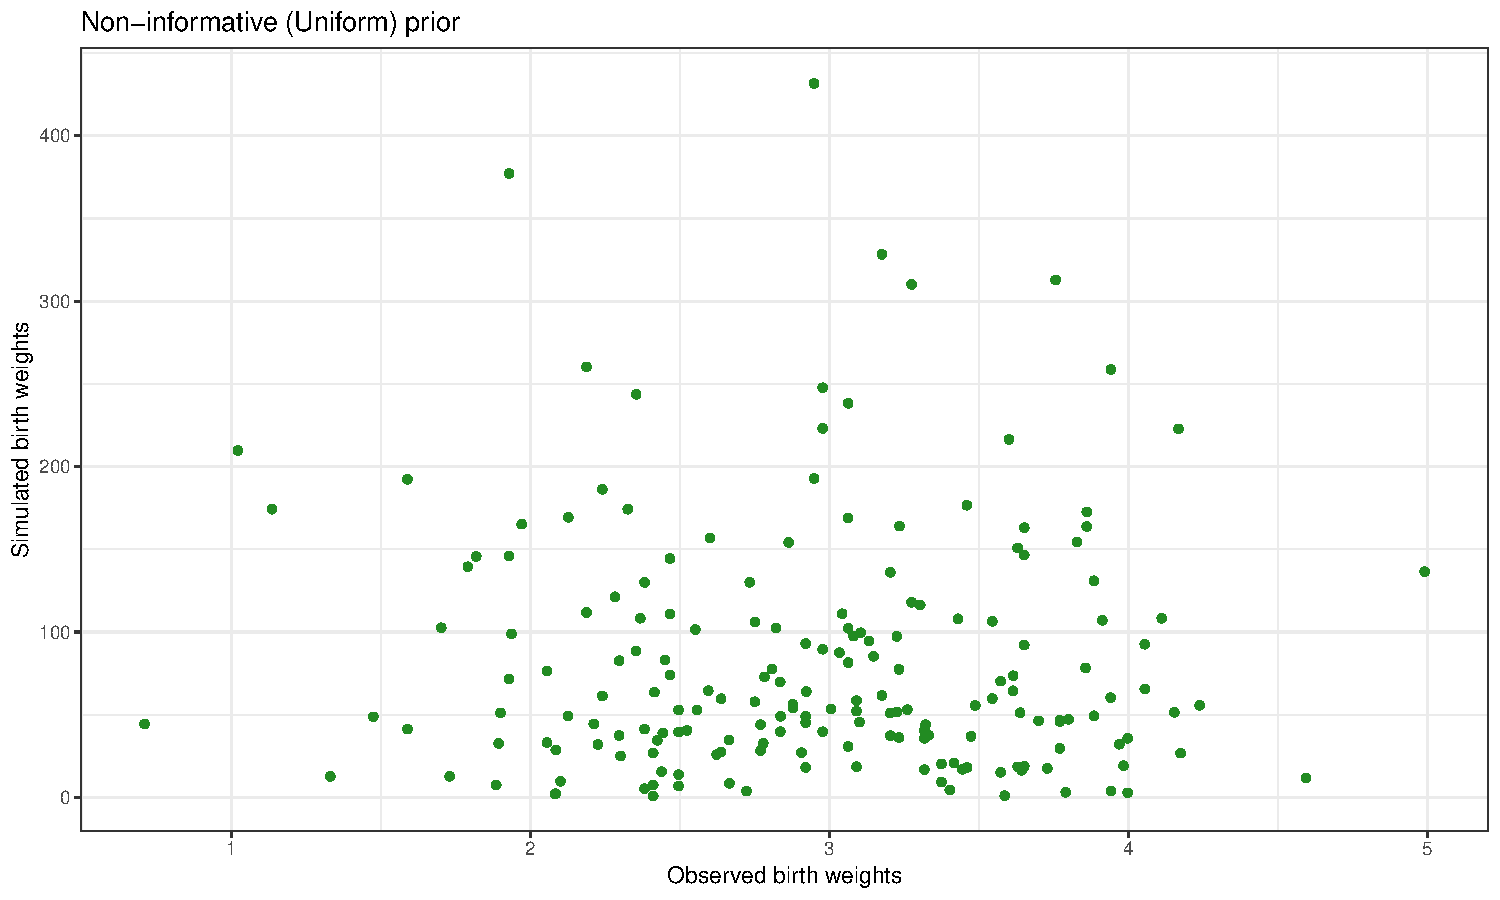
\includegraphics{DB_presentation_slides_files/figure-beamer/unnamed-chunk-5-1.pdf}

\end{frame}

\begin{frame}{2) Data simulation}

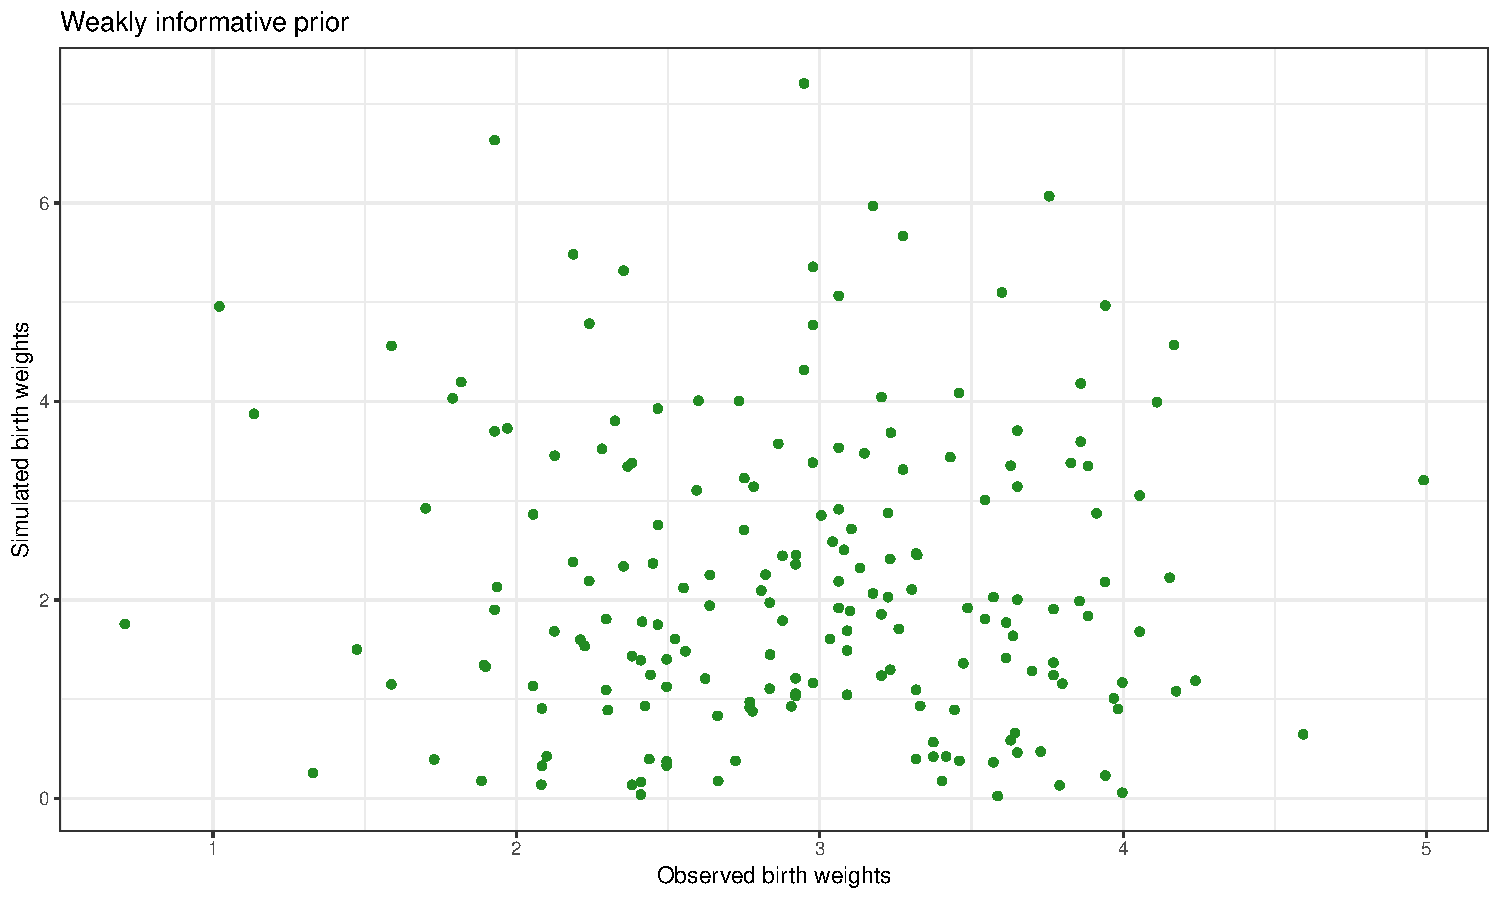
\includegraphics{DB_presentation_slides_files/figure-beamer/unnamed-chunk-6-1.pdf}

\end{frame}

\begin{frame}{3A) Model Fitting}

Once the simulated data are coherent with the observed data, it is
possible to proceed by fitting the model to the real data

\begin{itemize}
\setlength\itemsep{1em}
  \item{It is a good idea to put all the variables roughly on the
        unit scale}
  \item{Sampling from the posterior will require less computational
        effort and the algorithm will provide a more accurate 
        description of the surface of the posterior}
  \item{Some useful data pre-processing steps:}
  \begin{itemize}
    \item{Scale the variables by a constant, e.g. change unit of measure}
    \item{Trasform the covariates, e.g. log scale}
    \item{Use \textbf{QR} decomposition of the design matrix}
  \end{itemize}
\end{itemize}

\end{frame}

\begin{frame}{3B) MCMC algorithms}

\begin{itemize}
\setlength\itemsep{1em}
  \item{With very complex models with many parameters it is almost
        impossible to derive analytic form of the posterior}
  \item{Some algorithms that "explore" the posterior and sample from
        it are needed}
  \item{Markov Chain Monte Carlo (MCMC) are the most used algorithms,
        e.g. Metropolis-Hastings, Gibbs sampling}
\end{itemize}

\end{frame}

\begin{frame}{3B) MCMC algorithms}

\begin{itemize}
\item
  Hamiltonian Monte Carlo (HMC) algorithm has recently gained popularity
  because of its higher efficiency in sampling from the posterior with
  respect to Metropolis-Hastings and Gibbs sampling
\item
  \textbf{Stan} is an open-source software to perform Bayesian inferece
\item
  \textbf{Stan} uses the No-U Turn Sampler (NUTS), an efficient version
  of the HMC (Homan and Gelman 2014)
\end{itemize}

\end{frame}

\begin{frame}{3B) MCMC diagnostics}

\begin{itemize}
\setlength\itemsep{1em}
  \item{$R_{hat}$ ratio between the average variances of draws 
        within each chain to the variance of pooled draws across
        chains. If it converges to $1$ it means that the chains are
        in equilibrium}
  \item{Effective sample size (ESS) represents the number of samples
        that are actually independent. High number means less dependence
        between each state of the Markov chain and thus a better
        exploration of the posterior}
  \item{Divergent transitions of the MCMC algorithm}
\end{itemize}

\end{frame}

\begin{frame}{3B) MCMC diagnostics}

\includegraphics[width = 1.1\linewidth]{figures/div_trans.png}

\end{frame}

\begin{frame}{3B) MCMC diagnostics}

\begin{itemize}
\setlength\itemsep{1em}
  \item{MCMC diagnostics are fundamental to understand if the
        posterior has been adeguately explored}
  \item{If the sampling process did not perform well, biased inference
        will be obtained and the interpretation of such results
        could be misleading}
  \item{With complex models, reparameterize the model can be very
        helpful to ease the sampling process}
\end{itemize}

\end{frame}

\begin{frame}{4) Posterior calibration}

Does the data simulated from the model make sense with observed data?

\begin{itemize}
\setlength\itemsep{1em}
  \item{Plot the distribution of simulated data with the distribution
        of observed data}
  \item{Compare summary statistics of simulated and observed data}
  \begin{itemize}
    \setlength\itemsep{1em}
    \item{Mean and standard deviation}
    \item{Proportion of "special" values}
    \item{Quantiles}
\end{itemize}  
\end{itemize}

\end{frame}

\begin{frame}{4) Posterior calibration}

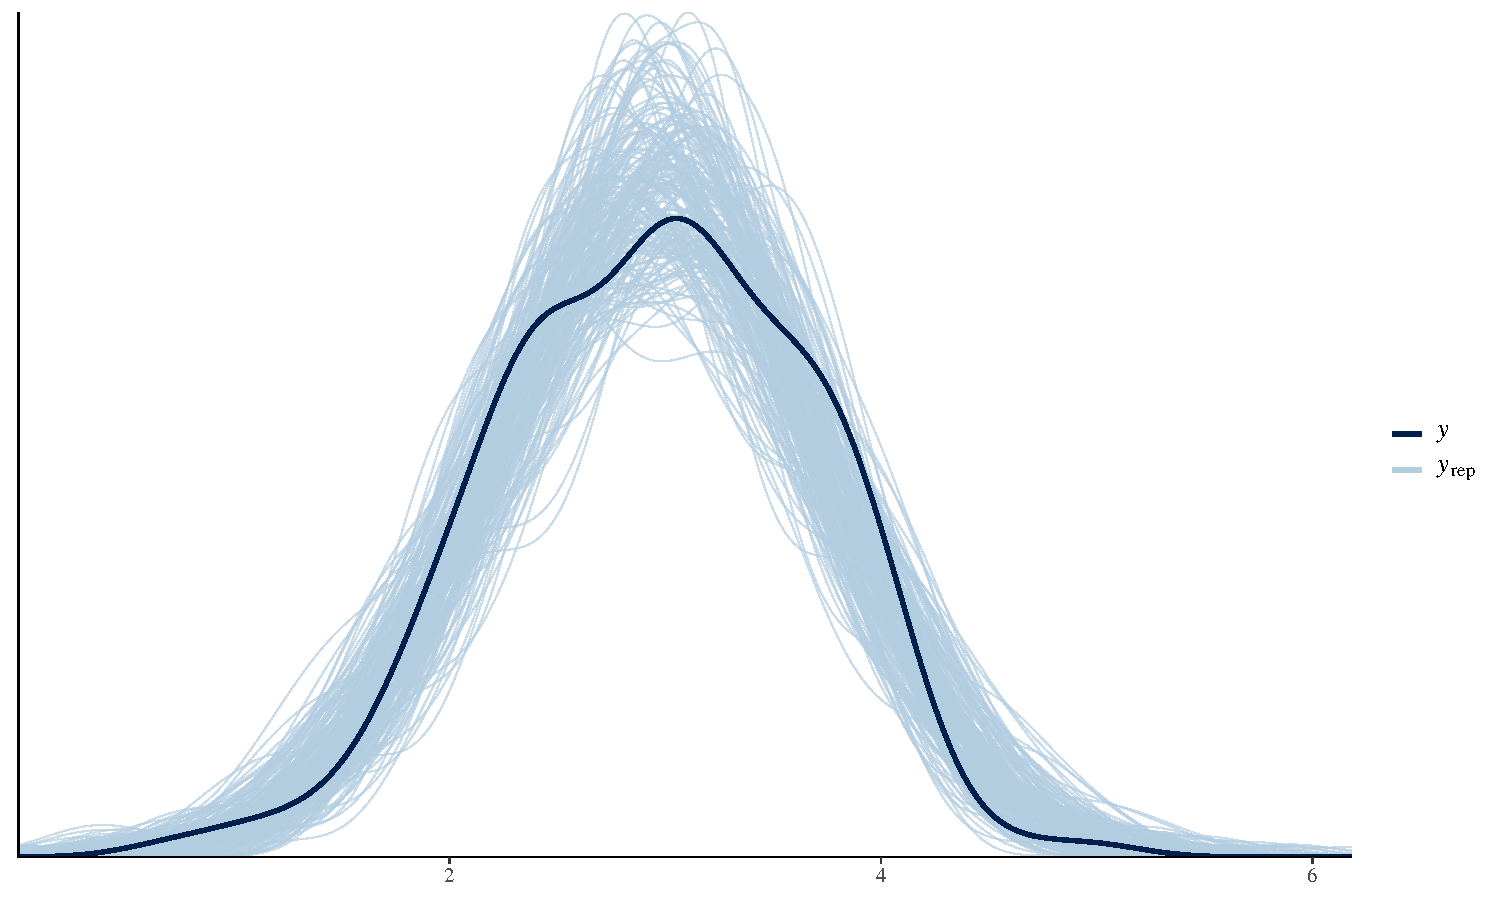
\includegraphics{DB_presentation_slides_files/figure-beamer/unnamed-chunk-7-1.pdf}

\end{frame}

\begin{frame}{4) Posterior calibration}

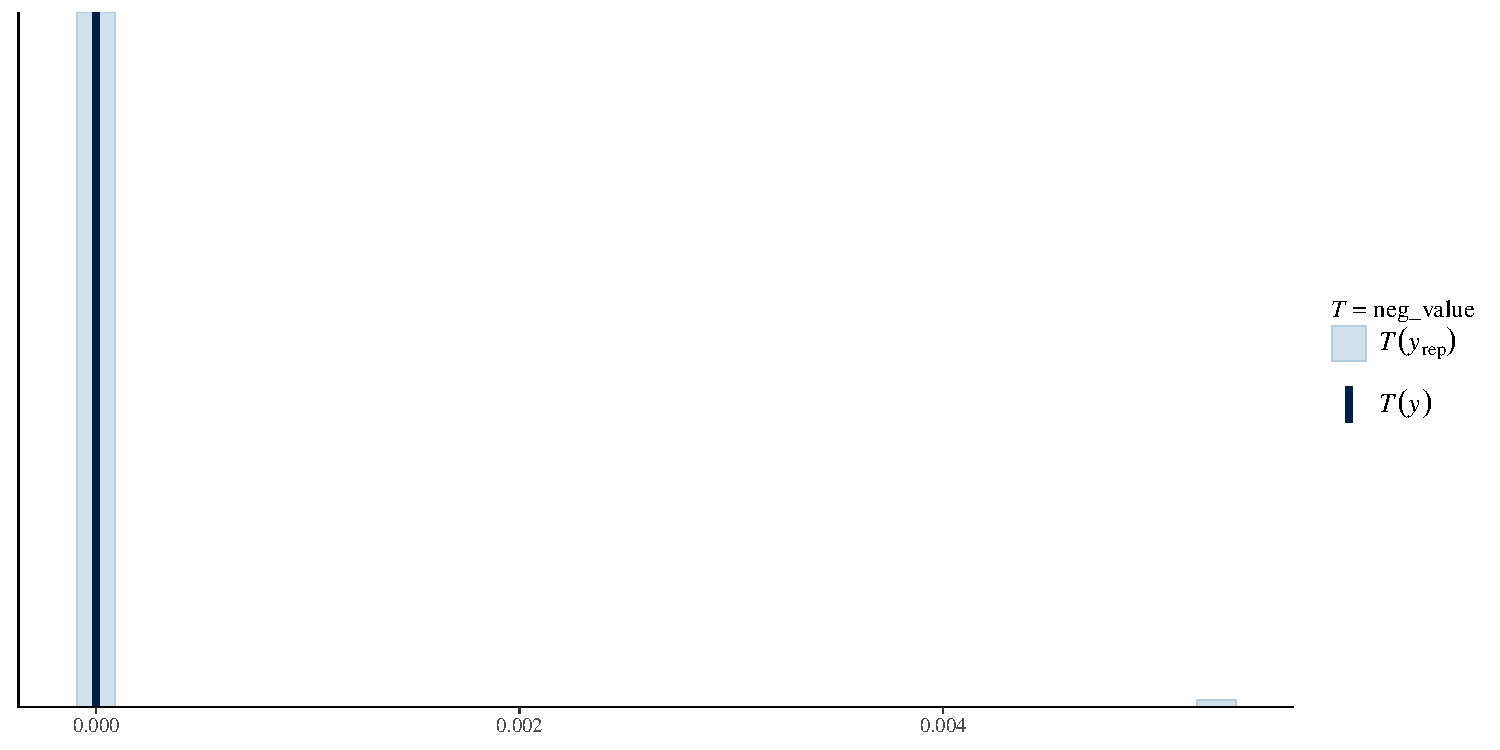
\includegraphics{DB_presentation_slides_files/figure-beamer/unnamed-chunk-8-1.pdf}

\end{frame}

\begin{frame}{4) Posterior calibration}

\begin{itemize}
\setlength\itemsep{1em}
  \item{Simulated data should not be identical to observed data}
  \item{They must range within plausible values of the analyzed data}
  \item{If simulated data are outside the range of plausible values
        or if they can't capture some features of the observed data,
        it would be a good idea to revise the model, e.g. change the
        family distribution}
\end{itemize}

\end{frame}

\begin{frame}{5) Model comparison}

\begin{itemize}
\setlength\itemsep{1em}
  \item{Identify which model best captures the features of the 
        observed data}
  \item{Leave-one-out cross-validation (LOO-CV) is used to evaluate
        the predictive distribution of each left-out data point}
  \item{The expected log predictive densities (ELPD) can be estimated
        using Pareto-smoothed importance sampling (PSIS)}
  \item{It can be also helpful to evaluate if there are some 
        observations that are influential for the log predictive
        density}
\end{itemize}

\end{frame}

\begin{frame}{5) Model comparison}

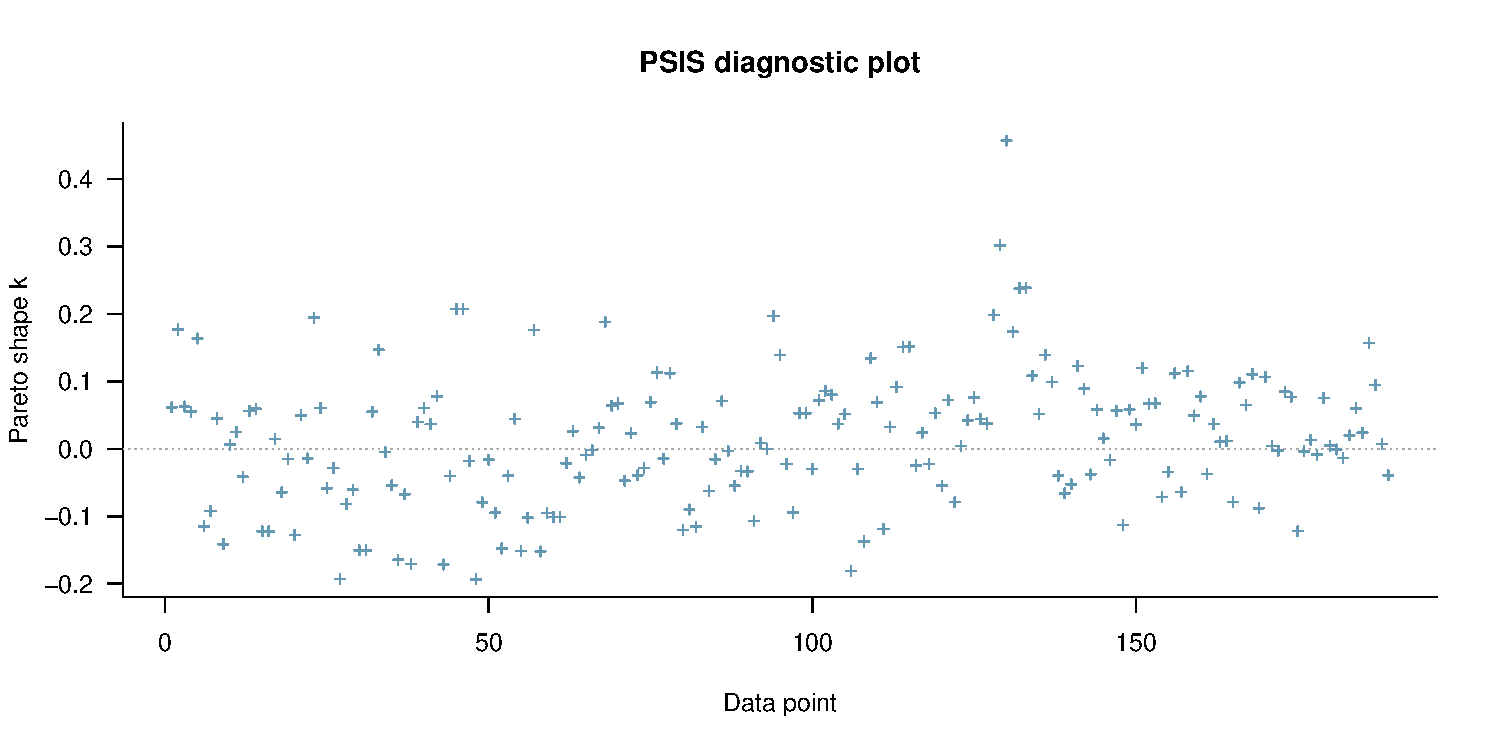
\includegraphics{DB_presentation_slides_files/figure-beamer/unnamed-chunk-9-1.pdf}

\end{frame}

\begin{frame}{5) Model averaging}

\begin{itemize}
\item
  Model averaging is a valuable alternative to model selection when more
  ``candidate'' models are present
\item
  Each model is weighted by its predictive performance (ELPD in the
  Bayesian context)
\item
  It can be very useful to evaluate which model has the higher ELPD,
  i.e.~higher weights in model averaging
\item
  Model averaging techniques (Yao et al. 2018):

  \begin{itemize}
  \tightlist
  \item
    \textbf{Pseudo bayesian model averaging (Pseudo-BMA)}
  \item
    \textbf{Pseudo bayesian model averaging with Bayesian Bootstrap
    (Pseudo-BMA BB)}
  \item
    \textbf{Stacking}
  \end{itemize}
\end{itemize}

\end{frame}

\begin{frame}{5) Model averaging}

\begin{longtable}[]{@{}lrrr@{}}
\caption{Model averaging with Stacking, Pseudo-BMA and Pseudo-BMA with
Bayesian Bootstrap.}\tabularnewline
\toprule
model & stacking & pseudo\_bma & pseudo\_bma\_bb\tabularnewline
\midrule
\endfirsthead
\toprule
model & stacking & pseudo\_bma & pseudo\_bma\_bb\tabularnewline
\midrule
\endhead
vague & 0.000 & 0.269 & 0.272\tabularnewline
weakly\_inf\_1 & 0.396 & 0.365 & 0.356\tabularnewline
weakly\_inf\_2 & 0.604 & 0.366 & 0.372\tabularnewline
\bottomrule
\end{longtable}

\end{frame}

\begin{frame}{Final remarks}

\footnotesize

\begin{itemize}
  \item{Prior distributions play a key role in the inference process,
        especially with complex and noisy data}
  \item{The ideal way to elicit prior distributions is to use 
        information from other studies or expert's opnions}
  \item{When the ideal derivation is challenging and time-consuming,
        priors should be calibrated given what we expect to observe}
  \item{The use of simulated data is crucial to understand and 
        calibrate a robust model for the data}
  \item{The sampling process must always be evaluate to avoid biased
        inference that could lead to unreasonable results}
  \item{We shouldn't be afraid of models with many parameters as long
        as they are built with regularizing (weakly informative) priors}
  \item{Combining inference from more than one model is valuable 
        approach to account for all the uncertainty the analyst has in
        the specific problem}
\end{itemize}

\end{frame}

\begin{frame}{References}

\scriptsize

\hypertarget{refs}{}
\hypertarget{ref-gelman_2004}{}
Gelman, Andrew. 2004. ``Exploratory Data Analysis for Complex Models.''
\emph{Journal of Computational and Graphical Statistics} 13 (4):
755--79.
doi:\href{https://doi.org/10.1198/106186004X11435}{10.1198/106186004X11435}.

\hypertarget{ref-gelman_2013}{}
Gelman, Andrew, John B. Carlin, Hal S. Stern, David B. Dunson, Aki
Vehtari, and Donald B. Rubin. 2013. \emph{Bayesian Data Analysis}. Third
Edition. Texts in Statistical Sciences. Chapman; Hall/CRC.

\hypertarget{ref-gelman_2017}{}
Gelman, Andrew, Daniel Simpson, and Michael Betancourt. 2017. ``The
Prior Can Often Only Be Understood in the Context of the Likelihood.''
\emph{Entropy} 19 (10). \url{http://www.mdpi.com/1099-4300/19/10/555}.

\hypertarget{ref-hoffman_2014}{}
Homan, Matthew D., and Andrew Gelman. 2014. ``The No-U-Turn Sampler:
Adaptively Setting Path Lengths in Hamiltonian Monte Carlo.'' \emph{J.
Mach. Learn. Res.} 15 (1): 1593--1623.
\url{http://dl.acm.org/citation.cfm?id=2627435.2638586}.

\hypertarget{ref-yao_2018}{}
Yao, Yuling, Aki Vehtari, Daniel Simpson, and Andrew Gelman. 2018.
``Using Stacking to Average Bayesian Predictive Distributions (with
Discussion).'' \emph{Bayesian Analysis} 13 (3): 917--1007.
doi:\href{https://doi.org/10.1214/17-BA1091}{10.1214/17-BA1091}.

\end{frame}

\end{document}
